% ============================================================
% CHAPITRE 5 : TESTS ET VALIDATION
% ============================================================
\chapter{Tests et validation}
\label{ch:tests}

Ce chapitre présente la stratégie de validation d'\AZIZA, couvrant les tests unitaires et d'intégration (117 tests automatisés), les tests fonctionnels de la plateforme web, et le protocole de test sur contractions réelles d'élèves.

\section{Tests unitaires et d'intégration}

Le pipeline \AZIZA\ est couvert par \textbf{117 tests unitaires et d'intégration}, répartis comme suit :

\begin{table}[h]
\centering
\caption{Répartition des 117 tests}
\label{tab:tests}
\begin{tabularx}{\textwidth}{l X r}
\toprule
\textbf{Module} & \textbf{Description} & \textbf{Nombre} \\
\midrule
Pipeline Forme & Métriques lexicales, syntaxe, orthographe & 45 \\
Pipeline Fond & Embedding, LLM, calibration & 25 \\
Pipeline Complet & Orchestration, verrous, fusion & 20 \\
Machine à états & Transitions, calcul M\(_p\), seuils & 15 \\
API REST & Endpoints, auth, rate limiting, erreurs & 7 \\
Interface Flask & Routes, templates, session & 5 \\
\midrule
\textbf{Total} & & \textbf{117} \\
\bottomrule
\end{tabularx}
\end{table}

Les tests d'intégration nécessitant l'API Mistral réelle sont marqués et peuvent être exclus lors des exécutions rapides. L'ensemble des tests est automatisé via GitHub Actions (CI) à chaque push.

\section{Tests Fonctionnels de la plateforme}
\label{sec:tests-fonctionnels}

Cette section présente les tests fonctionnels de la plateforme \AZIZA{} à travers trois aspects : la page d'évaluation, l'appel à l'API REST et l'affichage des résultats.

\subsection{Page d'évaluation}
\label{subsec:page-evaluation}

La page d'évaluation propose une interface utilisateur épurée permettant à l'apprenant de soumettre sa contraction. Elle se compose de deux zones de texte (texte source et contraction de l'apprenant), d'un sélecteur de mode (exercice/test) et d'un bouton de soumission. La figure~\ref{fig:page_evaluation} illustre cette interface.

\begin{figure}[H]
\centering
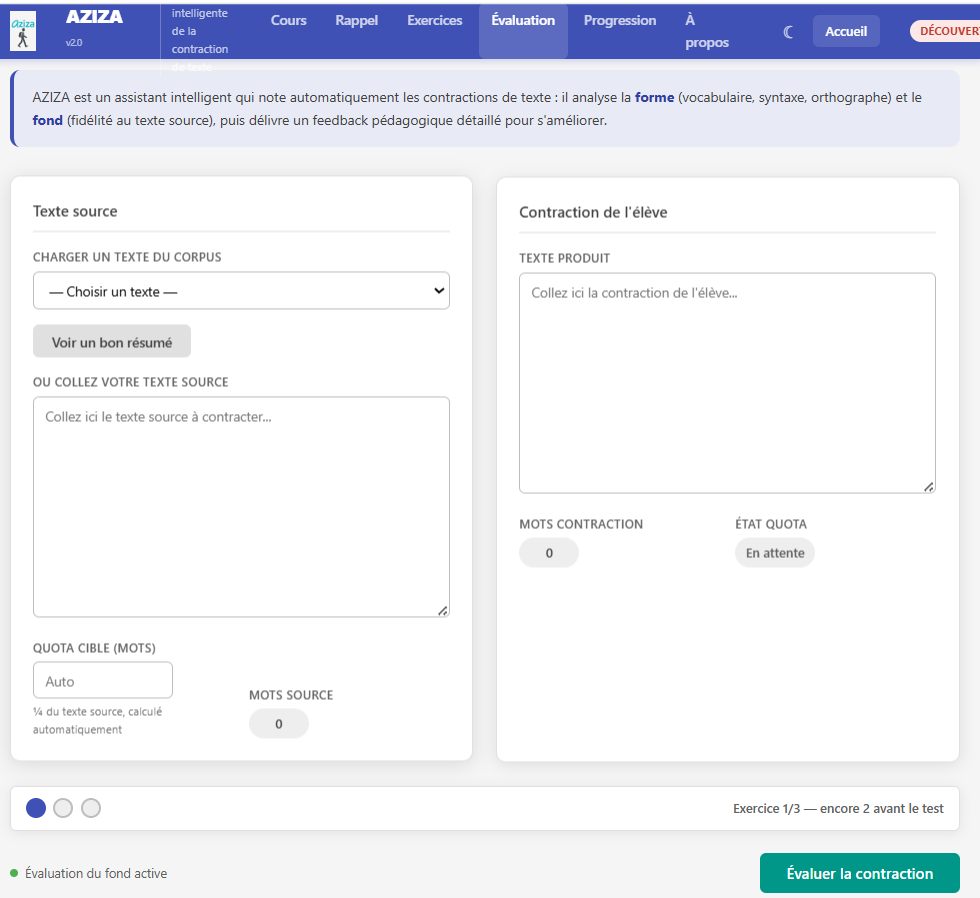
\includegraphics[width=0.95\textwidth]{page_evaluation.png}
\caption{Page d'évaluation de la plateforme AZIZA — formulaire de soumission}
\label{fig:page_evaluation}
\end{figure}

Le formulaire intègre une validation côté client (HTML5) et une vérification côté serveur via Flask-WTF. En cas d'erreur de saisie (champ vide, texte trop court), un message d'alerte s'affiche sans rechargement de page grâce à une requête AJAX.

\subsection{Test d'Appel à l'API}
\label{subsec:test-api}

L'API REST d'\AZIZA{} peut être testée indépendamment de l'interface web via un outil comme \texttt{curl} ou la documentation Swagger. L'appel suivant illustre une requête typique :

\begin{lstlisting}[caption=Test de l'API avec curl,language=bash]
curl -X POST https://Jiovany11.pythonanywhere.com/api/v1/evaluer \
  -H "Content-Type: application/json" \
  -H "X-API-Key: votre_cle_api" \
  -d '{
    "source": "Le texte source de reference...",
    "texte": "La contraction de l'apprenant...",
    "mode": "exercice"
  }'
\end{lstlisting}

La réponse JSON renvoyée contient la structure suivante :

\begin{lstlisting}[caption=Structure de la réponse JSON de l'API,language={}]
{
  "score_global": 6.5,
  "score_forme": 4.5,
  "score_fond": 2.0,
  "verrous": {"forme": true, "fond": false, "total": true},
  "feedback": {
    "erreurs": ["Idee principale omise"],
    "micro_cours": "Rappel : une contraction doit...",
    "exemple": "Voici une contraction correcte..."
  }
}
\end{lstlisting}

L'API retourne un code HTTP 200 en cas de succès, 400 pour une requête mal formée, 401 pour une clé API invalide et 429 en cas de dépassement du rate limiting. La documentation interactive Swagger est accessible via \texttt{GET /apidocs/}.

\subsection{Page des résultats}
\label{subsec:page-resultats}

Après soumission et traitement, la plateforme affiche une page de résultats synthétique et pédagogique. La figure~\ref{fig:page_resultats} présente cette interface.

\begin{figure}[H]
\centering
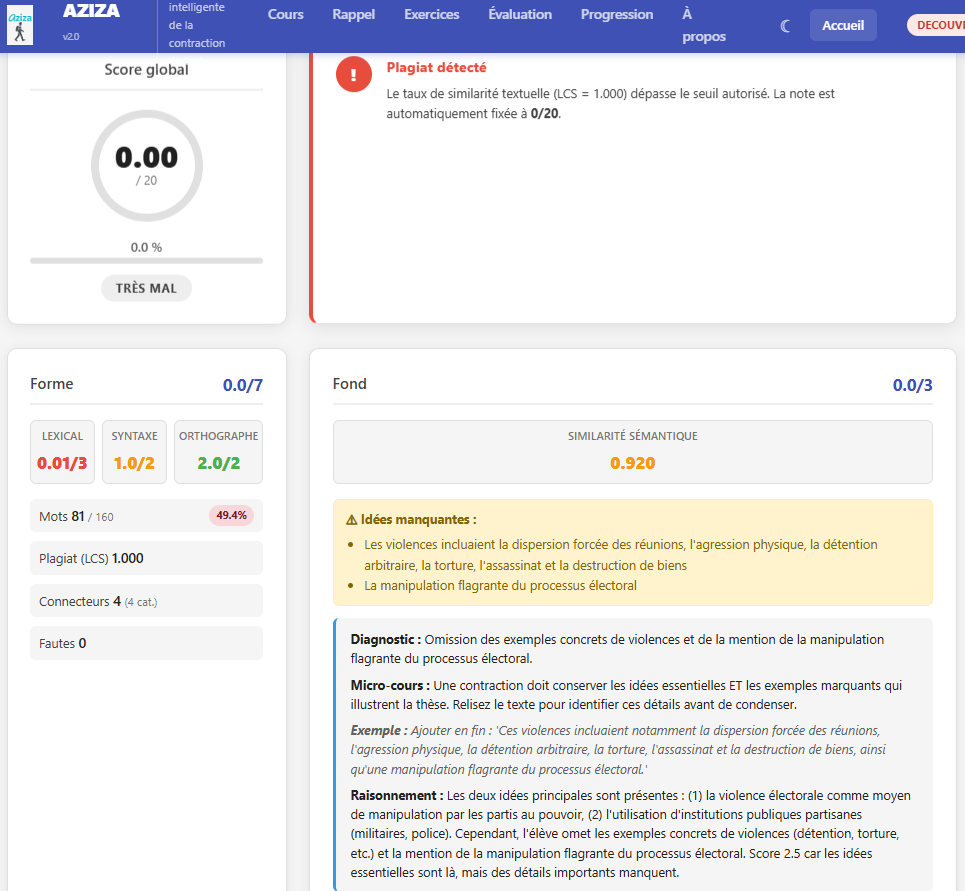
\includegraphics[width=0.95\textwidth]{page_resultats.png}
\caption{Page des résultats d'évaluation — scores et feedback pédagogique}
\label{fig:page_resultats}
\end{figure}

Le tableau de bord des résultats se compose de trois zones :
\begin{itemize}
    \item \textbf{Scores} : la note de forme (/7), la note de fond (/3) et le score total (/10) sont affichés avec un code couleur (vert si réussi, rouge si échoué).
    \item \textbf{Verrous pédagogiques} : chaque verrou (forme, fond, total) est représenté par une icône de validation ou d'échec, permettant à l'apprenant d'identifier rapidement ses axes d'amélioration.
    \item \textbf{Feedback Mistral} : la réponse du LLM est parsée et affichée sous forme de cartes structurées listant les erreurs détectées, les micro-cours correspondants et un exemple de contraction correcte.
\end{itemize}

L'ensemble de l'interface a été testé sur les deux terminaux décrits à la section~\ref{sec:ressources_materielles} (ordinateur portable et smartphone) afin de garantir une expérience utilisateur homogène quelle que soit la plateforme.

\section{Rapport de tests fonctionnels sur 10 contractions réelles}

\label{sec:tests_fonctionnels}

Cette section est réservée pour le rapport de tests fonctionnels comparant les performances d'\AZIZA\ à celles d'un correcteur humain sur 10 contractions réelles d'élèves de Terminale.

Le protocole prévu comprend :

\begin{enumerate}
    \item Sélection de 10 contractions anonymisées d'élèves de Terminale.
    \item Évaluation par un enseignant expert de français (note /10, feedback).
    \item Évaluation par le pipeline \AZIZA\ (note /10, feedback).
    \item Comparaison systématique : écart de note, concordance Kappa, analyse des divergences.
    \item Analyse qualitative des cas de désaccord (erreurs d'AZIZA, limites identifiées).
\end{enumerate}

% --- Contenu à compléter après expérimentation ---
\vspace{1cm}
\begin{tcolorbox}[colback=yellow!10,colframe=orange!80,title=\textbf{À COMPLÉTER}]
Ce rapport sera rédigé après la collecte des données expérimentales sur 10 contractions réelles d'élèves.
\end{tcolorbox}
\vspace{1cm}

Les résultats viendront compléter les métriques de validation du Chapitre~\ref{ch:experiences} et fourniront une indication concrète de la performance d'\AZIZA\ dans des conditions réelles d'utilisation.

\subsection*{Synthèse du chapitre}

Ce chapitre a détaillé la validation d'\AZIZA\ à trois niveaux : les 117 tests unitaires et d'intégration automatisés via GitHub Actions garantissent la robustesse du code ; les tests fonctionnels de la plateforme (page d'évaluation, appel API, page de résultats) valident l'expérience utilisateur sur terminal fixe et mobile ; le protocole de test sur 10 contractions réelles, dont les résultats sont à venir, permettra de confirmer la performance du pipeline en conditions réelles d'utilisation pédagogique.
